% Generated by experiments/make_article_assets.py from retained measurements.
% Edit the generator, not this fragment, to preserve reproducibility.
\subsection{Protocol, pairing, and completeness}

The retained run uses Python 3.12.14 on the recorded Linux
environment and contains 23 distinct supplied-sector cases,
46 case--protocol combinations, and 216 complete measured
arrangement/planar pairs. Each small combination has five measured
rounds; the principal family at $n\ge16$ has three. A round randomly
orders the arrangement arm, the planar arm, and a second identical
planar arm. Each protocol also records an excluded warmup for each
primary arm. Source construction, expected-list derivation, ray hashing,
independent coverage replay, and result serialization are outside the
timed intervals. Native coordinate validation remains inside enumeration.

There are 752 retained arm calls including warmups: 750 complete
and 2 resource-capped. All complete outputs agree with their case's
canonical primitive-ray digest. Separately, the independent exhaustive
checker returns \code{VERIFIED} for all 23 benchmark cases, including
the $n=32$ case whose arrangement warmups are capped. This replay is
outside both enumeration protocols. The additional high-size capability
runs below have their own, separately reported replay outcomes.

For complete matched rounds $i$, the reported ratio is
\[
 \rho=\operatorname{median}_i
       \left(\frac{T_i^{\mathrm{arrangement}}}{T_i^{\mathrm{planar}}}\right).
\]
The time columns show the separate median durations of the two arms.
Their quotient need not equal $\rho$: pairing is performed before
taking the median. Values above one favor the new enumerator. All
individual ratios and durations are retained; no ratio is assigned
when the baseline does not finish.

\subsection{The growing family and the removed work}

\begin{table}[htbp]
\centering\small
\setlength{\tabcolsep}{4pt}
\begin{tabular*}{\linewidth}{@{\extracolsep{\fill}}rr rrr rrr r@{}}
\toprule
& & \multicolumn{3}{c}{Prepared kernel} & \multicolumn{3}{c}{Build + enumerate} & \\
\cmidrule(lr){3-5}\cmidrule(lr){6-8}
$n$ & $t$ & Old (ms) & New (ms) & $\rho$ & Old (ms) & New (ms) & $\rho$ & Pairs\\
\midrule
1 & 3 & 3.026 & 1.718 & 1.82 & 2.894 & 1.735 & 1.71 & 5\\
2 & 4 & 7.921 & 2.045 & 3.84 & 7.818 & 2.358 & 3.59 & 5\\
4 & 6 & 44.521 & 2.931 & 15.18 & 46.822 & 3.763 & 12.10 & 5\\
8 & 10 & 490.356 & 5.076 & 95.15 & 491.897 & 6.269 & 78.16 & 5\\
16 & 18 & 10,219.114 & 11.955 & 924.16 & 9,648.874 & 15.511 & 626.20 & 3\\
32 & 34 & capped & 30.358 & --- & capped & 50.340 & --- & 0\\
\bottomrule
\end{tabular*}
\caption{Principal double-cap family, with cap types $(1,1)$ and
$t=n+2$ tetrahedra. Every complete list has seven non-link rays.
Times are median milliseconds; $\rho$ is the median matched ratio.
The pair count applies separately to each protocol. At $n=32$ there
are three completed new/new rounds per protocol and no completed
arrangement/planar pair.}
\label{tab:family-benchmark}
\end{table}

At $n=32$, the baseline warmup reaches the 15-second cooperative
wall-time allowance in each protocol. The driver does not repeat that
capped arm. It retains both unsuccessful warmups and reports the
complete new-arm times, with no speedup ratio. Every arm uses the
same clock policy, checked once per 256 callback invocations; the
allowance is cooperative rather than an exact preemptive timeout.

\begin{figure}[htbp]
\centering
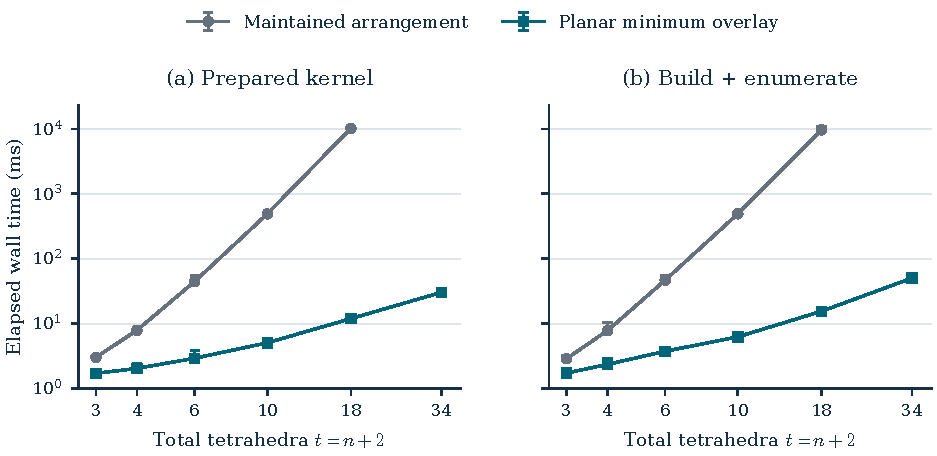
\includegraphics[width=\linewidth]{figures/paired_timings.pdf}
\caption{Observed complete-call medians for the principal family.
Whiskers show the full range of measured primary-arm replicates,
not confidence intervals. Both axes use logarithmic scaling.
The arrangement curve stops at $n=16$; its $n=32$ warmup was capped
and contributes no completed point. No asymptotic exponent is fitted.}
\label{fig:paired-times}
\end{figure}

The retained work counters give a concrete mechanism for the growing
difference. Table~\ref{tab:family-work} records completed prepared
calls. The maintained arrangement still has increasingly many equality
candidates to inspect and nonextreme positive candidates to reject.
Across these particular family instances, the planar diagram retains
three full-dimensional minimum cells and three internal segments, and
emits seven rays. These are measured instance counts; their finite
pattern is not used as a proof of an asymptotic family formula.

\begin{table}[htbp]
\centering\small
\begin{tabular*}{\linewidth}{@{\extracolsep{\fill}}rrrrrrrr@{}}
\toprule
& \multicolumn{4}{c}{Maintained arrangement} & \multicolumn{3}{c}{Planar overlay}\\
\cmidrule(lr){2-5}\cmidrule(lr){6-8}
$n$ & Planes & Bases & Positive & Nonextreme & Cells & Segments & Rays\\
\midrule
1 & 8 & 28 & 7 & 0 & 3 & 3 & 7\\
2 & 10 & 45 & 12 & 5 & 3 & 3 & 7\\
4 & 14 & 91 & 28 & 21 & 3 & 3 & 7\\
8 & 22 & 231 & 84 & 77 & 3 & 3 & 7\\
16 & 38 & 703 & 292 & 285 & 3 & 3 & 7\\
\bottomrule
\end{tabular*}
\caption{Exact counters from complete calls. ``Bases'' means attempted
arrangement bases; ``Positive'' includes candidates subsequently
rejected by the standard-ray rank filter. The new output has no final
rank-filter stage. Partial work at a cap is excluded from this table.}
\label{tab:family-work}
\end{table}

\subsection{Knot sources, controls, and timing noise}

For each listed frozen source, the driver maximizes
\[
 (\mathbf{1}_{\dim P=2},p,k,R,\text{support})
\]
lexicographically among the declared audited raw-nullity-three candidates.
This is a reproducible
selection rule for the stated stratum, with no claim of typical-knot
performance. The declared source \code{finite_trefoil} has no such
candidate and is explicitly skipped; its interior-subdivision source
does supply an eligible case. The three selected trefoil/figure-eight
sources in Table~\ref{tab:other-benchmarks} have zero essential-disc
rays in their frozen complete reference lists. Thus they also supply
negative disc-search controls at the supplied-sector level.

\begin{table}[htbp]
\centering\small
\setlength{\tabcolsep}{4pt}
\begin{tabularx}{\linewidth}{@{}Xrrrrrr@{}}
\toprule
& & & \multicolumn{2}{c}{Full median (ms)} & \multicolumn{2}{c}{Paired $\rho$}\\
\cmidrule(lr){4-5}\cmidrule(lr){6-7}
Source / control & $t$ & $R$ & Old & New & Prep. & Full\\
\midrule
Trefoil, interior subdivision & 8 & 7 & 10.715 & 3.426 & 3.84 & 3.14\\
Figure-eight & 10 & 7 & 17.835 & 4.176 & 5.73 & 4.18\\
Figure-eight, interior subdivision & 13 & 7 & 100.276 & 11.717 & 12.13 & 9.30\\
Solid torus $\#\mathbb{RP}^3$ & 5 & 7 & 6.648 & 2.582 & 2.63 & 2.40\\
Solid torus $\#(S^2\!\times S^1)$ & 7 & 7 & 21.271 & 5.503 & 4.64 & 3.87\\
\code{cap_1_2_3} & 4 & 7 & 5.866 & 3.444 & 1.76 & 1.71\\
\code{interior_3_5} & 6 & 2 & 7.531 & 1.515 & 6.42 & 4.90\\
Empty support & 3 & 0 & 0.098 & 0.100 & 0.48 & 0.94\\
One allowed type & 3 & 1 & 0.606 & 0.368 & 2.71 & 1.65\\
\bottomrule
\end{tabularx}
\caption{Selected frozen sources and small-query controls. Every row
has five complete pairs in each protocol and an independent exhaustive
replay. ``Full'' includes kernel construction; ``Prep.'' uses a common
prebuilt kernel. Exact source identifiers and supports are in the JSON.}
\label{tab:other-benchmarks}
\end{table}

All nine cap-type choices at $n=2$ are included in the retained data;
the $(1,1)$ choice is already part of the principal family and is
counted once. The empty-sector control was slower in this run:
its prepared median times are approximately $1.42\,\mu\mathrm{s}$
for the baseline and $3.56\,\mu\mathrm{s}$ for the new call. At this
scale individual durations are especially sensitive to measurement
noise. Its full-call ratio below one is retained rather than discarded.

The 222 identical-planar (A/A) ratios have median
$0.9967$, minimum $0.1426$, and maximum
$4.6486$. The two arms execute the same algorithm on the same
input, so these extremes demonstrate timing variation, not algorithmic
improvement. The minimum occurs in the empty-sector full control and
the maximum in a small cap-type full control. Every outlier remains in
the JSON. The sample sizes and this A/A spread support descriptive
comparisons for these cases, with no narrow confidence interval or
universal speedup claim.

\subsection{Separate capability runs and independent-replay limits}

The following larger principal-family cases receive one complete
new-only build-and-enumerate call each, with a 90-second cooperative
allowance. Their independent exhaustive replay has a separate
30-second allowance. These observations are neither paired timings
nor speedup measurements, and no baseline is extrapolated.

\begin{table}[htbp]
\centering\small
\begin{tabular*}{\linewidth}{@{\extracolsep{\fill}}rrrrrl@{}}
\toprule
$n$ & $t$ & Build (s) & Enumerate (s) & Total (s) & Independent replay\\
\midrule
64 & 66 & 0.158 & 0.152 & 0.310 & Verified (2.895 s)\\
128 & 130 & 0.954 & 0.409 & 1.364 & Verified (16.990 s)\\
256 & 258 & 7.868 & 2.332 & 10.199 & Capped (30 s); inconclusive\\
\bottomrule
\end{tabular*}
\caption{Single new-only capability observations, all returning seven
rays. The replay duration is outside the displayed total. The $n=256$
producer finishes, but the independent complete-list replay reaches its
separate cap; its coverage replay is therefore inconclusive.}
\label{tab:capacity}
\end{table}

At $n=256$, all returned rays pass the producer's native coordinate
validation, and the exact producer theorem applies under its stated
hypotheses. The timed experiment does not claim a completed independent
coverage replay for that case. This distinction exposes a practical
next target: after reducing enumeration work, dense preparation and
independent verification can become the dominant costs.

The authoritative observations, source hashes, canonical ray digests,
counters, arm orders, warmups, and limits are in
\code{results/paired_benchmark.json}; the compact comparison table is
\code{results/paired_benchmark.csv}. The reproduction driver is
\code{experiments/benchmark.py}. Figures and this input fragment are
regenerated by \code{experiments/make_article_assets.py}. Finite timing
data are used to evaluate the implementation on the declared inputs;
the asymptotic conclusions come from the proved bounds, and the global
unknot-recognition coverage problem remains separate.
